%%%%%%%%%%%%%%%%%%%%%%%%%%%%% TCC %%%%%%%%%%%%%%%%%%%%%%%%%%%%%%%%
%
% Template para TCC da Universidade Federal da Paraíba
%
% Autores: Elaine Soares elaineanita1@gmail.com
%          Rafael Brayner rafabrayner92@gmail.com
%          Roberto Júnior contato@robertojunior.net
%
% ShareLaTeX porting: Gustavo Sobral ghsobral@gmail.com
% 
% Revisão: Eudisley Anjos eudisley@ci.ufpb.br
%
% Sinta-se livre para melhorar e contribuir com esse projeto. 
%
%%%%%%%%%%%%%%%%%%%%%%%%%%%%%%%%%%%%%%%%%%%%%%%%%%%%%%%%%%%%%%%%%%%

\documentclass{tcc}

\begin{document}
\pagestyle{empty} %retira numeração da página
%Dados do TCC%
\author{Gabriel Machado Bandeira}
\title{Uma aplicação de Data Warehouse e mineração com base de dados de filmes}
\newcommand{\nomedocurso}{BACHARELADO EM CIÊNCIA DA COMPUTAÇÃO}
\newcommand{\orientador}{Prof. Dr. Jarley Palmeira Nóbrega}
\newcommand{\profa}{}
\newcommand{\profb}{}
\newcommand{\profc}{}
\newcommand{\insta}{\faculdade}
\newcommand{\instb}{\faculdade}
\newcommand{\instc}{\faculdade}
\newcommand{\coordenador}{Eduardo Calabria}
\newcommand{\departamento}{Nome do Departamento}

\begin{figure}[H]
\centering

\includegraphics[scale=2]{imagens/logo.png}
\end{figure}
\begin{center}
\textbf{\large{Faculdade Nova Roma}}\\
\textbf{\large{BACHARELADO EM CIÊNCIA DA COMPUTAÇÃO}}
\end{center}

\vspace{5em}

\begin{center}
\Large{\bf \MakeUppercase {\theauthor}}
\end{center}
\vspace{2em}
\begin{center}
\LARGE{\bf \MakeUppercase{\thetitle}}
\end{center}

\vfill






\vspace{2in}

\begin{center}
Recife, \MONTH, \the\year
\end{center}

\newpage
\begin{center}
\Large{\bf \MakeUppercase{\theauthor}}
\end{center}
\vspace{3in}
\begin{center}
\LARGE{\bf \thetitle}


\end{center}

\vspace{2in}

\begin{flushright}
Trabalho de Conclusão de Curso apresentado à \\Faculdade Nova Roma como pré-requisito parcial\\ para obtenção do título de Bacharel.\\
\vspace{0.2in}
Orientador: \orientador
\end{flushright}

\vfill
\begin{center}
\MONTH  de \the\year
\end{center}

\newpage
\begin{center}
\Large{\bf \MakeUppercase{\theauthor}}
\end{center}
\vspace{3in}
\begin{center}
\LARGE{\bf \thetitle}
\end{center}

\vspace{0.05in}

\begin{flushright}
Trabalho de Conclusão de Curso apresentado à\\ Faculdade Nova Roma como pré-requisito parcial\\ para obtenção do título de Bacharel, sob orientação\\ do \orientador
\end{flushright}

\vspace{0.7in}

\hrule
\noindent Prof. Dr. \profa\\
\insta\\

\vspace{0.25in}

\hrule
\noindent Prof. Dr. \profb\\
\instb\\

\vspace{0.25in}

\hrule
\noindent Prof. Dr. \profc\\
\instc\\


\newpage

%Agradecimentos%
\section*{\centering{AGRADECIMENTOS}} 
Gostaria de agradecer primeiramente a minha mãe, Maria Alessandra Vieira Machado, tia, Adriana Vieira Machado e irmã, Giovanna Paula Machado Bandeira, que sempre me apoiaram nos momentos mais difíceis e nunca saíram do meu lado.

As minhas amigas, Ana Maria Raymundi, Gabriela Lopes Vasconcellos de Andrade e Marina Schoepping Falcão Cavalcante Lins, que me deram muita força e ajuda para completar este trabalho.

A todos meus amigos e amigas que, direta ou indiretamente, contribuíram para a conclusão desse trabalho.

Ao meu orientador, Jarley Palmeira Nobrega, a todo apoio e incentivo que me ajudaram muito.

A Faculdade Nova Roma, pela oportunidade de fazer o curso.



\newpage

%Resumo%
\section*{\centering{RESUMO}}
O trabalho realizado neste documento foi de análise de dados, tratamento de dados e de tentar prever a nota de um filme com base em dados colhidos de outros filmes. O intuito desse trabalho é de que qualquer pessoa com interesse em mineração de dados possa usar os resultados aqui colhidos para poder expandir as conclusões que foram tiradas. Nesse trabalho foi possível concluir que prever a nota de um filme requer bastante análise dos dados. Foi possível prever a nota com um erro relativamente pequeno.

{\bf Palavras-chave:} $<$Mineração de Dados$>$,  $<$Aprendizado de Máquina$>$, $<$Pentaho$>$, $<$WEKA$>$.
\section*{\centering{ABSTRACT}} 
The work made in this document was data analysis, data treatment and try to predict the score of a movie based on the data gathered from other movies. The main goal of this work is that any other person that has an interest in data mining can use the data results genereted here to expand the conclusions made. In this work was possible to conclude that predict the score of a movie requires a lot of data analysis. It was possible to predict the score with a small error.

{\bf Key-words:} $<$Data Mining$>$, $<$Machine Learnning$>$, $<$Pentaho$>$, $<$WEKA$>$.
\newpage

%Lista de figuras%
\renewcommand{\listfigurename}{\centering LISTA DE FIGURAS}
\listoffigures
\newpage

%Lista de tabelas%
\renewcommand{\listtablename}{\centering LISTA DE TABELAS}
\listoftables
\newpage

%Lista de abreviaturas%
\section*{\centering{LISTA DE ABREVIATURAS}} 

DW	–  	Data Warehouse

PDI	– 	Pentaho Data Integration 

WEKA	–	Waikato Environment for Knowledge Analysis

MSE    –   Mean Squared Error

RMSE    –   Root Mean Squared Error



\newpage

%Sumário%

\pagestyle{plain} %mostra numeração da página%
\tableofcontents

\newpage
\section{INTRODUÇÃO}

Existem diversas fontes de dados que podem conter algum tipo de conhecimento que não está visível aos nossos olhos, um certo padrão que não é tão fácil reconhecer sem alguma computação. A mineração de dados pode reconhecê-los e nos ajudar a decidir o que fazer com eles, como deixar um produto mais próximo de outro em um supermercado, pois um algoritmo de mineração descobriu que esses dois produtos são geralmente comprados em conjunto.

A mineração de dados pode estar ligada à inteligência artificial, já que métodos de aprendizado de máquina podem ser utilizados para encontrar padrões e nos auxiliar a descrever melhor o que foi encontrado.
Pensando nisso, o objetivo deste trabalho é utilizar a mineração de dados em uma base do IMDB (\textit{Internet Movie Database}) para tentar encontrar padrões que possam nos ajudar a prever a nota de filmes do IMDB.

Vários fatores podem levar ao fracasso ou ao sucesso de um filme, como não escolher bem os diretores, os atores, pouco investimento etc. O IMDB contém informações de filmes, séries e animações, e para cada um desses existe uma nota relacionada. Essa nota é atribuída pelos usuários e é geralmente levada em consideração ao se escolher um filme, afinal, não é tão comum alguém querer assistir um filme que tem uma nota muito baixa.

A possibilidade de prever essa avaliação dos usuários seria uma ferramenta útil durante a produção de um novo filme, os estúdios não gostariam que os seus filmes tenham péssimas avaliações e já podem trabalhar em cima do que foi previsto e possivelmente melhorar a nota.

Para isso, a mineração de dados irá se basear em dados históricos dos filmes para buscar encontrar algo que possa ajudar a melhorar a nota de um filme. Esse algo pode ser uma diretora especifica, línguas em que o filme foi lançado etc.

Visto isso, algumas hipóteses foram levantadas e os modelos foram usados para validá-las (ou não).

Para prever a nota de um filme baseado em dados históricos, aqui será discutido sobre a criação de Data Warehouses, que utiliza o processo de ETL (\textit{Extract, Transform, Load}), que será aplicado nesse trabalho, para serem criados. CRISP-DM, metodologia usada na mineração de dados e com uma visão de Bussiness Intelligence e uma ferramenta para auxiliar o ETL, o \pdi, junto com a linguagem de programação \textit{Python}.

Aqui também terá uma pequena introdução ao WEKA (\textit{Waikato Environment for Knowledge Analysis}), uma poderosa ferramenta para mineração de dados, com diversas formas de aplicar algoritmos em cima dos dados construídos.

Nesse capítulo, a motivação e os objetivos do trabalho foram apresentados. No Capítulo 2, uma visão geral sobre Data Warehouse será mostrada. No Capítulo 3, as principais características da plataforma Pentaho Data Integration serão introduzidas. Um breve resumo sobre o mineração de dados e a ferramenta WEKA é mostrado no Capítulo 4. O Capítulo 5 apresenta a metodologia utilizada no estudo de caso e também exibe e discute os principais resultados obtidos. A conclusão desse trabalho é apresentada no Capítulo 6.

\section{Fundamentação Teorica}
\subsection{Data Warehouse}
\subsubsection{Definição}
Para \citeAuthorPageYear{jmj}, um \textit{Data Warehouse} é um repositório de informações coletadas de múltiplas fontes, armazenado sobre um esquema definido e, geralmente, situado em um único local, no intuito de garantir a consistência dos dados caso eles sejam acessados de locais diferentes. Eles suportam o processamento de informações ao prover uma plataforma sólida de dados históricos para análise.

\subsubsection{Características de um Data Warehouse}
Segundo \citeAuthorPageYear{inmon}, um DW (Data Warehouse) é um conjunto de dados orientado por assuntos, integrado, variável com o tempo e não volátil, criados para dar suporte à decisão.

Para \citeAuthorPageYear{jmj}, é orientado por assunto, ou seja, organizado em torno de um assunto principal. Em vez de se concentrar nas operações diárias e no processamento de transações de uma empresa, um DW foca na modelagem e análise de dados para tomadores de decisões. 
Integrado, um DW contém informações de fontes heterogêneas, como base de dados relacionais e \textit{flat files}. Processos de \textit{data integration} e \textit{data cleaning} são aplicados para garantir a consistência dos dados.

Variável com o tempo, armazena informações históricas dos últimos 5-10 anos, por exemplo. Toda estrutura chave em um DW contém um elemento de tempo.
E por último, não volátil, os dados não precisam ser alterados, já que um DW é fisicamente separado do ambiente operacional. As únicas operações executadas em um DW são: carga inicial e acesso aos dados \citep{jmj}.

\subsubsection{Modelos de Data Warehouse}
Para \citeAuthorPageYear{jmj}, um DW pode ser dividido em três modelos: \textit{enterprise warehouse}, \textit{data mart} e \textit{virtual warehouse}.

\subsubsection{Enterprise Warehouse}
\citeAuthorPageYear{jmj} diz que um \textit{enterprise warehouse} coleta informações sobre um assunto que abrange toda uma organização. Ele fornece integração de dados em escala corporativa, geralmente de um ou mais sistemas operacionais ou de provedores de informação externos. Ele contém dados detalhados e sumarizados e podem variar de alguns poucos \textit{gigabytes} para centenas de \textit{gigabytes}.

Um \textit{enterprise warehouse} é um conglomerado das \textit{data warehouse staging} e \textit{presentation areas} de uma organização \citep{kimball2002}


\subsubsection{Data Mart}
Conforme \citeAuthorPageYear{jmj} diz, um \textit{data mart} contém um subconjunto de dados de uma escala corporativa e tem o escopo limitado a assuntos específicos.

Os \textit{data marts} são frequentemente implementados em servidores de baixo custo e têm o seu ciclo de implementação medido em semanas, em vez de meses ou anos. Os dados podem ser independentes ou dependentes. Caso sejam independentes, vão ter como fonte um ou mais sistemas operacionais ou provedores de informação externos. No caso de serem dependentes, os dados contidos no \textit{data mart} serão fornecidos diretamente de um \textit{enterprise warehouse}.

\subsubsection{Virtual Warehouse}
\citeAuthorPageYear{jmj} dizem que as \textit{virtual warehouses} são um conjunto de \textit{views} em cima dos bancos de dados operacionais. Eles podem manter um processamento eficiente de \textit{queries} exibindo apenas alguns dos possíveis sumários. Ele também é de fácil construção.

\subsubsection{Componentes}

A figura \ref{dwComponents} mostra quais são os componentes de um DW, explicados com detalhes mais abaixo.
\begin{figure}[H]
\centering
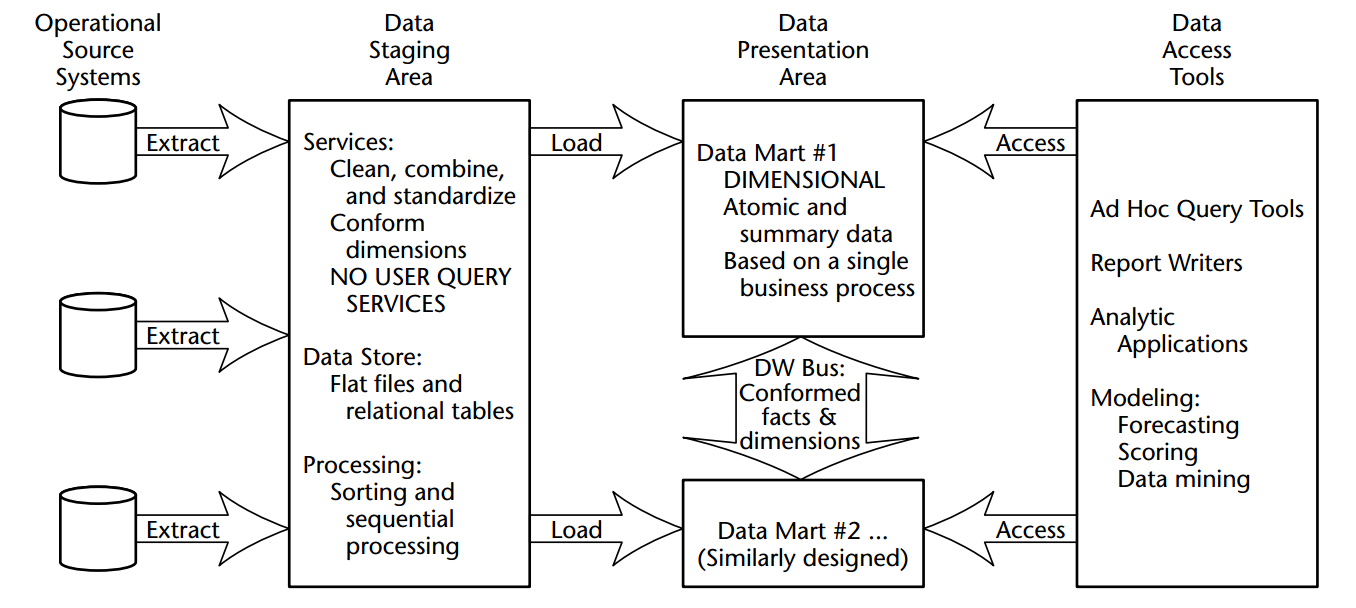
\includegraphics[height=5cm]{imagens/componentes_DW.png}
\caption{Componentes de um Data Warehouse (\citeauthor{kimball2002} \citeyear{kimball2002})}
\label{dwComponents}
\end{figure}

\subsubsubsection{Operational Source Systems}
Fontes de Dados Operacionais, nas palavras de \citeAuthorPageYear{kimball2013}, são responsáveis pela captura de transações de negócio. Esses sistemas são mantidos fora do \textit{data warehouse} porque se tem pouco ou nenhum controle sobre o conteúdo ou formato dos dados. Eles processam performance e disponibilidade. Eles também afirmam que esses sistemas mantêm poucos dados históricos. Um bom \textit{data warehouse} pode reduzir a necessidade dos sistemas de dados operacionais de representarem o passado. Em muitos casos, eles são de algum propósito especial, sem responsabilidade de compartilhar dados comuns, como dados de produtos, clientes etc.

\subsubsubsection{Data Staging Area}
\citeAuthorPageYear{kimball2002} sugerem que a \textit{staging area} é tanto uma área de armazenamento como um conjunto de processos conhecidos como \textit{extract, transformation, loading} (ETL). Esse processo será melhor explicado mais pra frente. Eles ainda falam que a \textit{staging area} é tudo entre os \textit{operational source systems} e a \textit{presentation area}. 

Existem diversas formas de carregar dados na \textit{staging area}, como \textit{flat files}, xml, modelos relacionais. Ela regularmente é composta de um \textit{database management system} (DBMS) e arquivos de texto (\textit{flat files}) \citep{kimball2004}. Em muitos casos, os dados precisam ser armazenados fora de um DBMS, em \textit{flat files}, para um rápido processamento sequencial.
\citeAuthorPageYear{kimball2002} descrevem o primeiro passo na criação (extração) de um \textit{data staging area} como ler e entender da fonte de dados e copiar o que for necessário para manipulação futura. Afirma que quando os dados são extraídos, existem diversas transformações que podem ser feitas, como limpeza, combinação de dados de diferentes fontes, remoção dados duplicados etc. Essas transformações acontecem antes de se carregar os dados na \textit{presentation area}.

\subsubsubsection{Data Presentation Area}
A \textit{presentation area}, ou área de apresentação, é onde os dados estão organizados, armazenados e disponíveis para consulta por usuários ou alguma aplicação analítica de \textit{Business Intelligence} (BI), de acordo com \citeAuthorPageYear{kimball2013}. Tudo que o negócio vê e toca é através das ferramentas de acesso ou aplicações de BI.

Os dados devem ser, de acordo com \citeAuthorPageYear{kimball2013}, apresentados, armazenados e acessados através de esquemas dimensionais, sejam eles esquemas estrela ou cubos OLAP (\textit{online analytical processing cubes}), que são modelos dimensionais de alta performance implementados em \textit{softwares} de proposito especial. Eles devem conter dados atômicos detalhados. Embora a \textit{presentation area} contenha dados agregados, é completamente inaceitável que somente dados sumarizados sejam armazenados enquanto os dados atômicos estão trancados em modelos normalizados. Os dados mais finamente granulados devem ser apresentados na \textit{presentation area} para que usuários possam fazer as perguntas mais precisas.

A área de apresentação deve ser estruturada ao redor dos processos de medição de eventos. \citeAuthorPageYear{jmj} dizem que os modelos dimensionais devem corresponder aos eventos de captura de dados, não devem entregar um "relatório do dia". 

\subsubsubsection{Data Access Tools} Ferramentas de Acesso de Dados, ou \textit{Data Access Tools}, são ferramentas usadas para consultar área de apresentação. Uma ferramenta dessas, de acordo com \citeAuthorPageYear{kimball2013} pode ser tão simples quanto \textit{Queries Ad Hoc}, \textit{queries} usadas para determinado proposito e usadas quando se tem a necessidade, ou tão complexa quanto uma ferramenta de mineração de dados ou modelagem. 

\subsubsection{Extract, Transform, Load (ETL)}
O processo de \textit{extract, transform, load} (extrair, transformar, carregar), mais conhecido como ETL, é um processo utilizado para a construção de um DW, contendo os passos que são mostrados na figura \ref{etl}. 
\begin{figure}[H]
\centering
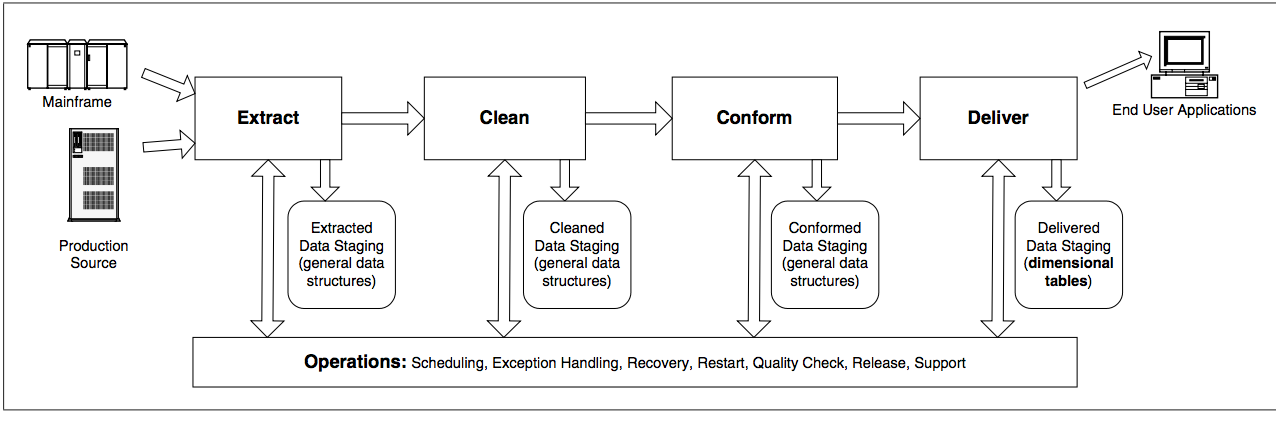
\includegraphics[height=5cm]{imagens/dw_process.png}
\caption{Processo de ETL (\citeauthor{kimball2004} \citeyear{kimball2004})}
\label{etl}
\end{figure}
O primeiro passo é a extração dos dados: espera-se que o sistema extraia dados de uma grande variedade de fontes, segundo \citeAuthorPageYear{kimball2013}. As organizações podem extrair dados de fontes como arquivos xml, banco de dados, planilhas etc.

O segundo passo é a transformação: \citeAuthorPageYear{kimball2013} dizem que após os dados serem extraídos, diversas transformações podem ser executadas, como limpeza, que irá remover alguns ruídos, combinação de dados de fontes diversas (bancos de dados, \textit{data warehouses}, arquivos csv, planilhas, etc) e tratar dados duplicados. Essa limpeza pode mudar os dados e aperfeiçoar o seu valor para uma organização.

O terceiro e último passo é o carregamento, que é o processo de estruturar fisicamente e carregar os dados dentro dos modelos dimensionais da \textit{presentation area}, de acordo com \citeAuthorPageYear{kimball2013}.

\subsubsection{Modelagem Dimensional}
\citeAuthorPageYear{DWlifecycle} afirma que modelagem dimensional é uma técnica de design lógico para estruturação de dados de forma que seja intuitivo para os usuários do negócio e que tenha uma performance rápida de \textit{querys}.

Ele ainda afirma que essa modelagem é amplamente aceita. Os dados apresentados devem ser simples, para que tenham alguma chance de sucesso. A simplicidade é um requerimento fundamental, porque garante que os usuários irão entender os bancos de dados, segundo \citeAuthorPageYear{DWlifecycle}.

Existem quatro etapas para a construção de um modelo dimensional, sendo elas:

\begin{itemize}
    \item selecionar o processo de negócio
    \item declarar o grão
    \item identificar as dimensões
    \item identificar os fatos 
\end{itemize}

Segundo \citeAuthorPageYear{kimball2013}, os processos de negócio são as atividades operacionais realizadas por uma organização. É um processo importante, pois define como o grão, dimensões e fatos serão declarados. O grão estabelece o que uma única linha na tabela de fatos representa.

\subsubsubsection{Tabela de Dimensões}
De acordo com \citeAuthorPageYear{kimball2013}, as dimensões fornecem o contexto de "quem, o que, onde, quando e como" de cada processo do negócio. As tabelas de dimensões podem incluir diversas colunas, mas costumam ter menos dados que a tabela de fatos. Elas têm chave primária, que vai permitir o relacionamento com a tabela de fatos.
A tabela de dimensões pode ser conhecida como a "alma" de um sistema de DW, pois contém dados que permitem que o sistema de DW seja alavancado.

\subsubsubsection{Tabela de Fatos}
Para \citeAuthorPageYear{kimball2013}, a tabela de fatos armazena as métricas resultantes de um processo de negócio de uma organização. Cada linha em uma tabela de fatos representa um evento de medição. Os dados, em um nível especifico de detalhe, podem ser chamados de grãos, como apenas uma linha por produto vendido.

Os dados mais úteis são os numéricos e aditivos. Aditividade é importante, pois dificilmente irá se fazer uma consulta que traga apenas uma linha, mas sim trará centenas, milhares ou milhões de dados e a coisa mais útil para se fazer com eles é somar.

\citeAuthorPageYear{kimball2013} falam que é possível manter dados textuais em uma tabela de fatos, eles são comumente usados para descrever algo e estão em uma lista discreta de valores. 

As tabelas de dimensões, conforme \citeAuthorPageYear{kimball2013}, têm uma ou mais chaves estrangeiras, que irá se ligar as chaves primarias das tabelas de dimensões. Eles afirmam que a tabela de fatos tem sua própria chave estrangeira, que é um subconjunto das chaves estrangeiras, chamado de chave composta. 

\subsubsubsection{Esquema Estrela}
Esse esquema, mostrado como exemplo na figura \ref{star}, armazena os dados em uma arquitetura semelhante a uma estrela, onde cada ponta é uma dimensão e todas se relacionam com a tabela de fatos, como mostra a figura. \citeAuthorPageYear{jmj} mostram que a tabela de fatos contém chaves para todas as outras tabelas assim como dados de medidas.
\begin{figure}[ht]
\centering
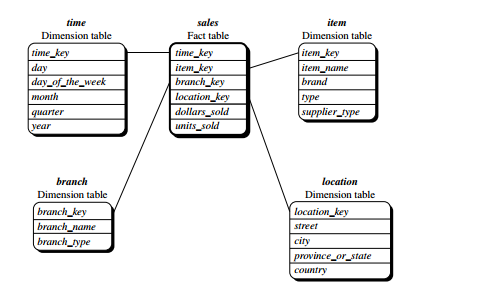
\includegraphics[height=6.2cm]{imagens/starscheme.png}
\caption{Esquema Estrela (\citeauthor{jmj} \citeyear{jmj})}
\label{star}
\end{figure}
\\
\subsubsubsection{Esquema Snowflake}
Como mostra na figura \ref{snowflake}, o esquema \textit{snowflake} é uma variação do esquema estrela onde algumas tabelas de dimensões são normalizadas, ou seja, dividindo os dados em tabelas adicionais, segundo \citeAuthorPageYear{jmj}.
\begin{figure}[ht]
\centering
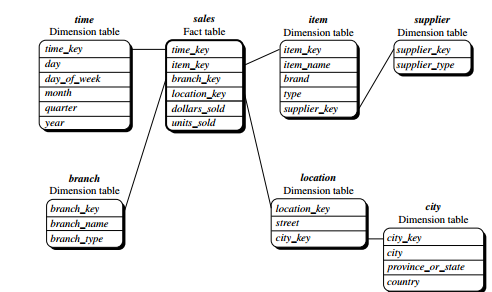
\includegraphics[height=6.2cm]{imagens/snowflakescheme.png}
\caption{Esquema Snowflake (\citeauthor{jmj} \citeyear{jmj})}
\label{snowflake}
\end{figure}
\subsubsubsection{Cubo e OLAP}
Conforme \citeAuthorPageYear{jmj}, DW e ferramentas OLAP são baseados no modelo multidimensional e ele visualiza os dados no formato de cubos de dados, como mostra a figura \ref{cube}. Um cubo permite visualizar os dados em diversas dimensões simultaneamente.
\begin{figure}[ht]
\centering
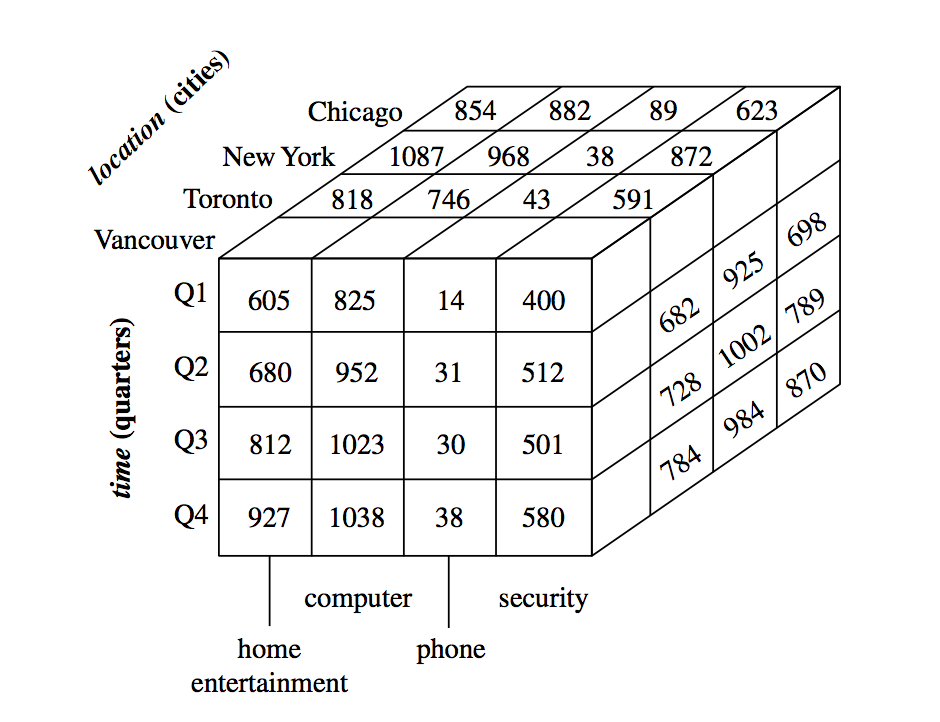
\includegraphics[height=6.2cm]{imagens/datacube.png}
\caption{Exemplo de um cubo de dados (\citeauthor{jmj} \citeyear{jmj})}
\label{cube}
\end{figure}
Dimensões são entidades que uma organização quer manter os dados. Uma dimensão deve ter uma tabela associada, a tabela de dimensões.


\citeAuthorPageYear{kimball2013} dizem que os modelos dimensionais implementados em base de dados multidimensionais são chamados de \textit{online analytical processing cubes} (OLAP). Diversas operações estão associadas a esses cubos, como \textit{roll up, drill down, slice and dice e pivot}

\begin{itemize}
    \item \textbf{roll-up}: segundo \citeAuthorPageYear{jmj}, a operação de \textit{roll-up} executa agregações em um cubo de dados ou por \textit{subir em uma hierarquia conceitual} de uma dimensão ou por redução dimensional. Quando essa operação é realizada, uma ou mais dimensões podem ser retiradas do cubo.
    
    \item \textbf{drill-down}: De acordo com  \citeAuthorPageYear{jmj}, essa operação é a inversa da \textit{roll-up}, indo de dados menos detalhados para dados mais detalhados. Pode ser feito ou por \textit{descer uma hierarquia conceitual} de dimensões ou \textit{introduzir dimensões adicionais}
    
    \item \textbf{slice and dice}: Segundo  \citeAuthorPageYear{jmj}, a operação \textbf{slice} faz uma seleção em uma subdimensão do cubo, resultando em um subcubo. A operação \textbf{dice} cria um subcubo ao efetuar uma seleção em uma ou mais dimensões.
    
    \item \textbf{pivot}: \citeAuthorPageYear{jmj} dizem que \textit{pivot} (ou rotate) é uma operação que permite mover o cubo em algum eixo permitindo uma exibição dos dados em de uma forma alternativa.
\end{itemize}

\subsection{Pentaho Data Integration}
Nas seções anteriores discutiu-se um pouco sobre as principais características de um Data Warehouse. Nessa seção, será discutida o uso do PDI no processo de ETL, como ela pode ser aplicada e suas principais características.
O PDI (\textit{\pdi}), também conhecido como Kettle, oferece diversas ferramentas para a extração de dados de fontes diversas, transformações, limpezas e de carregamento dos dados
\subsubsection{Arquitetura}
O \pdi é composto basicamente de quatro componentes:
\begin{itemize}
    \item Spoon: é uma aplicação \textit{desktop} de interface gráfica para a criação de \textit{jobs} e \textit{transformations}. Permite a criação de processos de ETL sem a necessidade de programação;
    \item Pan: uma interface de linha de comando que pode ser usada para a execução de \textit{transformations} e \textit{jobs} criados no \textit{spoon};
    \item Kitchen: interface de linha de comando que pode ser usada para a execução de \textit{jobs};
    \item Carte: uma aplicação \textit{web} que é capaz usar um servidor de ETL remoto, fornecendo capacidades de execução remota similares ao servidor de \textit{Data Integration}.
\end{itemize}

\subsubsection{Princípios de Design}
\citeAuthorPageYear{kettle} afirmam que o Pentaho foi desenvolvido com alguns princípios de design fundamentais. Algumas experiências negativas levaram a essas decisões. São eles:

Ele é de fácil desenvolvimento, não é preciso se preocupar com instalação do \textit{software}. Uma das facilidades do \pdi é que não é necessário programar, pois toda linha de código adiciona complexidade e custo de manutenção, como por exemplo  várias ferramentas baseadas em Java precisavam que o usuário especificasse explicitamente qual era o nome da Classe Java do Driver e a URL do JDBC, caso tenha uma conexão com o banco de dados. 

O \pdi mantém as funcionalidades disponíveis na interface de usuário, \citeAuthorPageYear{kettle} afirmam que é possível realizar o processo de ETL utilizando arquivos XML, repositório ou uma API, e todas essas opções estão disponíveis em uma interface gráfica. O \pdi não tem limitações de nomenclatura, ou seja não é necessário se preocupar com restrições como tamanho e escolha de caracteres.

\citeAuthorPageYear{kettle} falam que deixar que qualquer pessoa veja o que está acontecendo nas várias partes de um processo de ETL é crucial, pois oportuniza acelerar o desenvolvimento e reduzir o custo. Ele tem um fluxo de dados flexível, o \pdi foi criado para ser o mais flexível possível, respeitando os fluxos que são criados, é possível distribuir ou copiar dados por diversos \textit{steps} como escrever em arquivos de texto ou incluir em bases de dados relacionais. E por fim, apenas mapear dados impactados, todos os campos que não são mapeados passam automaticamente para o próximo passo do processo, reduzindo assim o custo de manutenção.

O \pdi contém uma série de nomenclaturas que são utilizadas para se referir a algo que faz parte de sua arquitetura:

Começando com \textit{transformations}, \citeAuthorPageYear{kettle} dizem que as transformações manipulam os dados de um processo de ETL. Ele consiste de um ou mais \textit{steps} que realiza leitura, limpeza e ou carregamento dos dados em outra base de dados. Esses \textit{steps} estão conectados através de \textit{hops}.

Os \textit{steps}, de acordo com \citeAuthorPageYear{kettle}, são o bloco de construção principal em uma \textit{transformation}. Um \textit{step} contém um nome único, ele pode ler e escrever dados, eles podem escrever dados em um ou mais \textit{hops}. 

Além disso tudo, cada \textit{step}, segundo \citeAuthorPageYear{kettle} possui uma funcionalidade distinta, seja ela de ler dados, escrever dados, realizar transformações e etc. Os \textit{transformation hops}, para \citeAuthorPageYear{kettle}, representam o caminho dos dados entre os \textit{steps}. 





\subsection{Mineração de Dados}

O termo mineração de dados, de acordo com \citeAuthorPageYear{jmj} poderia ter sido chamado de mineração de conhecimentos dos dados, já que minerar é um processo para encontrar pequenas quantidades de preciosidades de uma grande quantidade de material bruto. 

Outros dizem que mineração de dados é um sinônimo de KDD (\textit{knowledge discovery from data}), descobrimento de conhecimento a partir de dados. A mineração também é vista como um passo essencial no processo de descoberta de conhecimento, como mostra a figura \ref{kdd}. 


\begin{figure}[H]
\centering
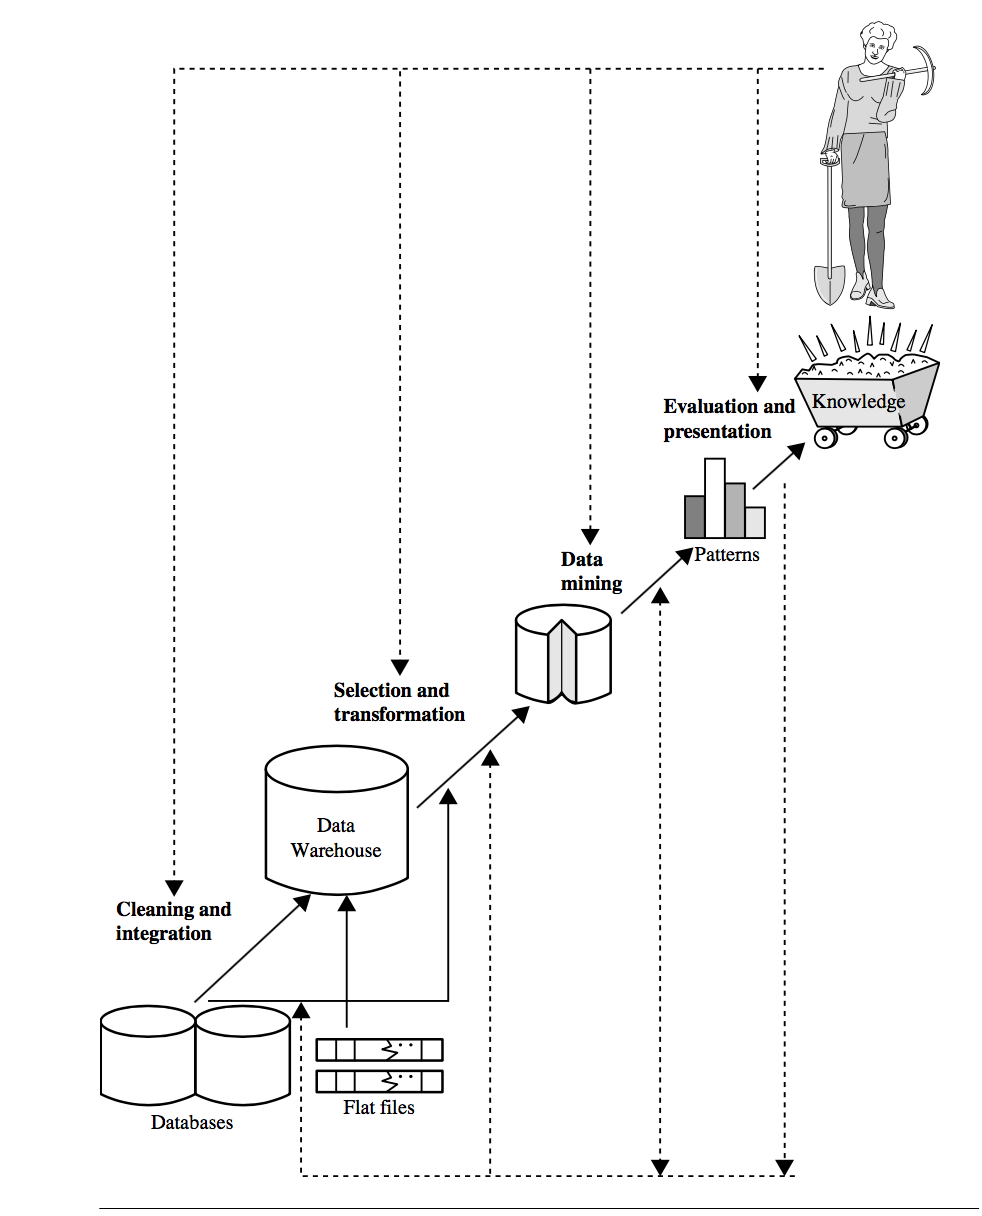
\includegraphics[height=9cm, width=9cm]{imagens/kdd.png}
\caption{Mineração de dados como um processo de descoberta de conhecimento \citep{jmj}}
\label{kdd}
\end{figure}

\citeAuthorPageYear{advancedDM} afirmam que massas de dados gerados de caixas registradoras, de bases de dados específicas, etc são exploradas, analisadas, reduzidas e reusadas. Ainda dizem que pesquisas são feitas através de diversos modelos para prever vendas, resposta de mercado, lucro, etc

Já \citeAuthorPageYear{jmj} afirmam que a mineração de dados tem diversas funcionalidades, como caracterização (sumarização das características gerais de uma classe alvo de dados) e discriminação (comparação das características gerais de uma classe alvo com as características de uma ou mais classes diferentes). 

Também é usada para encontrar padrões que aparecem frequentemente nos dados. Existem alguns tipos de padrões, como \textit{frequent itemset}, itens que geralmente aparecem juntos em um conjunto de dados transacionais, \textit{frequent subsequence} ou \textit{sequencial pattern}, que, por exemplo, é o padrão de um cliente que compra primeiro um \textit{notebook}, seguido de uma câmera digital e então um cartão de memória, de acordo com \citeAuthorPageYear{jmj}. Por último, tem as \textit{frequent substructures}, que são formas estruturadas que aparecem frequentemente, como grafos e árvores, que podem conter \textit{itemsets} e \textit{subsequences}.

Algoritmos de classificação, regressão, etc são usados para análises preditivas, tentando prever dados categóricos ou discretos. A classificação, segundo \citeAuthorPageYear{jmj}, é o processo de encontrar um modelo que melhor expressa uma classe. Esse modelo é derivado da análise de um conjunto de treinamento. Os modelos são representados usando árvores de decisão, fórmulas matemáticas, redes neurais etc.

Já a regressão, o uso mais comum é para tentar prever valores numéricos contínuos, com algoritmos como regressão linear, regressão LASSO etc.

De acordo com \citeAuthorPageYear{jmj}, também existem os algoritmos de clusterização, que, diferentemente da classificação e regressão, analisam os dados sem consultar as suas classes. Em alguns casos, os dados até vem sem classe. A clusterização é usada para encontrar classes para os grupos de dados. Os \textit{clusters} são formados de uma forma que os objetos dentro deles tenham uma grande similaridade ao se compararem uns com os outros, mas se diferenciam dos objetos em outros \textit{clusters}.

\subsubsection{CRISP-DM}
\subsubsubsection{Definição}
CRISP-DM, ou\textit{ Cross-industry standard process for data mining}, é uma técnica aplicada no processo de mineração de dados, com uma série de tarefas a serem realizadas para chegar ao melhor resultado.
Segundo \citeAuthorPageYear{dmfd}, a mineração de dados não é algo feito uma vez e depois esquecido, o trabalho pode ser aplicado em outros projetos, servir de referência.
O ciclo de vida da mineração de dados contém seis fases, como apresentado na figura \ref{crispcycle}: entendimento do negócio, entendimento dos dados, preparação dos dados, modelagem, avaliação e implementação. 
A mineração de dados não termina uma vez que a solução é implementada.
\begin{figure}[H]
\centering
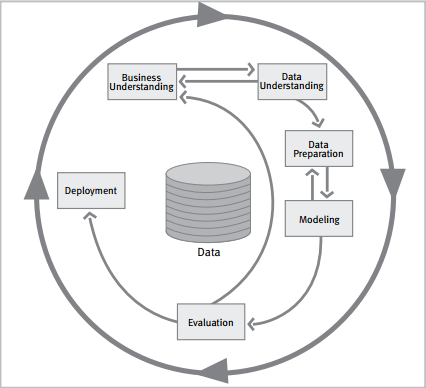
\includegraphics[height=6.2cm]{imagens/lifecycle.png}
\caption{Ciclo de vida (\citeauthor{crispmanual} \citeyear{crispmanual})}
\label{crispcycle}
\end{figure}
As fases tem diversas tarefas que são realizadas para completa-las e toda tarefa tem suas saídas. \citeAuthorPageYear{advancedDM} afirmam que esse processo não é rigio e precisa ser seguido ao pé da letra, além de que nem todos os processos precisam ser utilizados, caso a pessoa já tenha alguma experiência.
\subsubsubsection{Entendimento do negócio}
A primeira etapa do CRISP-DM é o entendimento do negócio, que foca em esclarecer os objetivos do negócio e seus requerimentos de uma perspectiva de negócio.

O primeiro objetivo da análise de dados é entender, sob uma perspectiva de negócio, o que o cliente deseja realizar. Segundo \citeAuthorPageYear{dmfd}, deve-se ter um entendimento claro do problema que se deseja abordar, o objetivo do negócio, as limitações e o impacto. Esse processo produz uma informação da situação do negócio, objetivo do cliente e o critério de sucesso.

Em seguida é realizada uma avaliação da situação. Segundo \citeAuthorPageYear{crispmanual}, essa tarefa consiste em um detalhamento maior dos recursos, limitações, premissas e outros fatores que devem ser considerados ao determinar os objetivos da análise de dados e do plano de projeto.

Outra etapa é determinar os objetivos da mineração de dados, por exemplo, como "prever quantas pessoas irão visitar uma loja no verão, de acordo com informações dos últimos 2 anos dessa loja".

E então produzir plano de projeto, ou seja, de acordo com \citeAuthorPageYear{crispmanual}, o plano desejado para atingir os objetivos da mineração de dados e desse modo, os objetivos do negócio. Esse processo produz o plano de projeto e avaliações iniciais de ferramentas e técnicas.

\subsubsubsection{Entendimento dos dados}
De acordo com \citeAuthorPageYear{dmfd}, na segunda etapa do projeto de mineração de dados, os dados têm que ser obtidos e deve-se verificar se eles são apropriados para as necessidades.

A primeira tarefa desse processo é coletar dados iniciais e então realizar, caso necessário, o carregamento dos dados em alguma ferramenta. Nessa tarefa é produzida uma lista de todos os \textit{datasets} adquiridos, junto com localizações, métodos realizados para coleta e problemas encontrados.

A próxima tarefa é descrever os dados, explora-se eles usando técnicas de visualização. Essa análise esta diretamente ligada aos objetivos da mineração de dados , de acordo com\citeAuthorPageYear{crispmanual}. Essa tarefa produz um relatório da exploração de dados, contendo descobertas iniciais ou hipóteses, e o seu impacto no restante do projeto.

Depois, é necessário verificar a qualidade dos dados, respondendo perguntas como "os dados estão completos?", "existem valores faltantes?". É criado um relatório da qualidade dos dados, com uma lista de problemas encontrados e suas soluções.

\subsubsubsection{Preparação dos Dados}
A maior parte do tempo gasto no processo de mineração de dados é na preparação deles, já que diversos tratamentos precisam ser feitos nos dados e isso nem sempre é tão simples. De acordo com \citeAuthorPageYear{dmfd}, a maior parte dos dados usados para mineração foi originalmente coletada e preservada para outros objetivos e precisa ser refinada antes de ser ficar pronta para a modelagem.

Essa parte tem duas saídas, antes das tarefas, que são: \textit{datasets}, dados produzidos e que serão usados para modelagem e \textbf{descrição do \textit{dataset}}.

A primeira tarefa é \textbf{selecionar os dados} que serão usados na modelagem, baseando-se nos objetivos da mineração de dados, qualidade e limites técnicos, segundo \citeAuthorPageYear{crispmanual}. É criada uma lista de dados que foram incluídos e excluídos e a razão para isso.

Segundo \citeAuthorPageYear{crispmanual}, Posteriormente é feita uma \textbf{limpeza dos dados}, que eleva a qualidade dos dados para o nível requerido pelas técnicas de análise selecionadas. De acordo com \citeAuthorPageYear{dmfd}, dificilmente os dados selecionados estarão perfeitamente limpos, mudanças precisarão ser feitas nos dados para atingir o nível necessário. Transformações nos dados são feitas para limpeza e possível impacto na análise de resultados. Nessa etapa é criado um relatório de limpeza de dados: que descreve as ações tomadas para lidar com os problemas encontrados anteriormente.

A tarefa seguinte é \textbf{Construir dados}, que consiste na criação de novos campos, dados agregados, ou novos formatos de dados. É produzida uma lista de atributos derivados a partir dos que já existem e explica como e por que eles foram gerados e uma lista de registros criados, junto com o motivo e como eles foram formados.

A próxima tarefa é \textbf{integrar dados}, já que existe a possibilidade deles estarem em diferentes \textit{datasets} e é necessário a integração desses dados para a próxima etapa, modelagem. A saída desse passo é: \textbf{dados fundidos}: fundir tabelas se refere a juntar duas ou mais tabelas que têm diferentes informações sobre o mesmo objeto. 

Por último, a tarefa \textbf{formatar dados} é aplicada. Dados frequentemente vêm em formatos que não são os convencionais para modelagem, segundo \citeAuthorPageYear{dmfd}, então conversões precisam ser feitas. O processo de preparação de dados deve ser finalizada com um \textit{dataset} pronto para modelagem e um relatório descrevendo o \textit{dataset}.

A saída é dados reformatados, convertidos para alguma unidade de medida única para todos os dados (como quilos, em peso).

\subsubsubsection{Modelagem}
É a etapa na qual alguma técnica de aprendizado de máquina é aplicada, testada e avaliada para encontrar padrões nos dados, como \textit{K-nearest neighbors}, \textit{Decision Tree }e etc. Dependendo do tipo de dados, diversos modelos podem ser aplicados, de acordo com \citeAuthorPageYear{advancedDM}.

O primeiro passo da modelagem é \textbf{selecionar a técnica de modelagem} que será usada. De acordo com \citeAuthorPageYear{crispmanual}, caso múltiplas técnicas sejam aplicadas, é preciso executar essa tarefa para cada uma delas. Nem todas as técnicas de modelagem serão úteis para as necessidades do negócio.

A escolha da técnica de modelagem depende muito dos tipos de dados, as técnicas, de acordo com \citeAuthorPageYear{advancedDM}, podem ser de associação, clusterização, previsão, etc.

De acordo com \citeAuthorPageYear{advancedDM}, em associação, a relação entre um item em uma transação de dados com outros itens, nessa mesma transação, é usada para prever padrões.

Na clusterização, segundo \citeAuthorPageYear{advancedDM}, dados não agrupados são agrupados utilizando técnicas automatizadas. Já a previsão é relacionado a técnicas de regressão. A ideia é descobrir a relação entre variáveis dependentes e independentes. Utilizando dados históricos, as técnicas de regressão, sejam lineares ou não, podem gerar uma curva de regressão que pode ser usada para realizar previsão.

Em seguida, o \textbf{teste de design} é gerado, ou seja, procedimentos ou mecanismos para testar a qualidade e validade do modelo, segundo  \citeAuthorPageYear{crispmanual}. Os dados geralmente são separados em dois conjuntos, o de treinamento e o de teste. O de treinamento é usado para construir o modelo e o de teste para validar ele. Nessa etapa é gerado descrito como planeja, treina, testa e avalia o modelo.

Depois, \citeAuthorPageYear{crispmanual} afirmam que é o momento de \textbf{construir o modelo}, rodar a ferramenta de modelagem para criar um ou mais modelos. Esse processo produz um documento com as configurações de parâmetros usados, modelos produzidos pela ferramenta e uma descrição deles.

Por fim, é a fase de \textbf{avaliar o modelo}, que sumariza os dados e ranqueia os modelos e também revisa as configurações dos parâmetros aplicados para tentar reajustá-los até encontrar a melhor possível.

\subsubsubsection{Avaliação}
Avaliar todo o processo: não só os modelos, mas também o processo empregado para a sua criação.

A primeira tarefa é \textbf{avaliar resultados}. Ela avalia o grau em que o modelo se adequa ao objetivo original do negócio e busca determinar se existe alguma razão para o modelo estar deficiente.

Ela também avalia o resultado da mineração de dados a respeito do critério de sucesso do negócio, \citeAuthorPageYear{dmfd} mostra que esse processo serve para dizer se o projeto atingiu ou não os objetivos definidos no início e seleciona os modelos que atingiram o critério selecionado.

Após a última tarefa, é feita uma \textbf{revisão do processo}, nesse ponto, os modelos resultantes aparentam ser satisfatórios para a necessidade do negócio, segundo \citep{crispmanual}. Essa é um passo usado para rever o processo, como algum problema que foi negligenciado. \citeAuthorPageYear{crispmanual} mostram que se deve sumarizar a revisão e ressaltar as atividades que não foram realizadas e aquelas que devem ser repetidas.

De acordo com \citeAuthorPageYear{dmfd}, a última fase é \textbf{determinar próximos passos}. A fase de avaliação é concluída com as recomendações para o próximo passo. Decidir se deve finalizar o projeto ou continuar o desenvolvimento. Para \citeAuthorPageYear{crispmanual}, essa fase também inclui a análise das despesas e recursos restantes, que tem influencia na decisão.
Essa etapa produz uma lista de possíveis ações e a decisão.

\subsubsubsection{Implementação}
O objetivo dessa última parte é a implementação do modelo.
O primeiro passo, de acordo com \citeAuthorPageYear{crispmanual} é o plano de implementação, usando os resultados da avaliação e determina a estratégia de implementação. 

A primeira parte é gerar um plano que sumariza as estratégias para implementação, os passos necessários e como realizar.
Posteriormente é feito um \textbf{Plano de monitoramento e manutenção}, conforme \citeAuthorPageYear{dmfd} diz, a mineração de dados é um ciclo, então existe a necessidade continuar envolvida com os modelos enquanto eles são integrados ao dia-a-dia. Para \citeAuthorPageYear{crispmanual}, a preparação cuidadosa das estratégias de manutenção ajuda a evitar longos períodos desnecessários de uso incorreto dos resultados da mineração.

Em seguida é produzido um plano de monitoramento e manutenção que sumariza todas as estratégias de manutenção e monitoramento, incluindo os passos necessários para realizá-los.
Em seguida, é feito um \textbf{Relatório Final}, um sumário do projeto e das experiências ou uma apresentação final e compreensível dos resultados da mineração.
Essa etapa produz o relatório final, que sumariza todo o projeto ao juntar todos os relatórios criados até o momento, de acordo com \citeAuthorPageYear{dmfd} e apresentação final, um encontro realizado na conclusão do projeto com seu cliente.

Por último, é feita uma \textbf{revisão do projeto} na qual o time se reúne e discute o que deu e não deu certo, o que pode e não pode ser feito novamente, e coisas que devem ser evitado.
A saída é uma documentação de experiência que sumariza a experiência ganha com o projeto, como erros e acertos, dicas de como selecionar os melhores modelos para situações semelhantes etc.

\subsubsection{WEKA}

O WEKA, \textit{Waikato Environment for Knowledge Analysis}, segundo \citeAuthorPageYear{weka}, é uma coleção de algoritmos de aprendizado de máquina e de ferramentas de preprocessamento de dados. Ele é criado de uma forma que os algoritmos possam ser testados rapidamente nos \textit{datasets}. Também contém suporte de mineração de dados, como preparação dos dados, avaliar modelos estatisticamente, visualização dos dados e resultados da aprendizagem. Todas essas ferramentas estão disponíveis em uma interface simples. O WEKA é escrito em Java e é distribuído sob a GNU \textit{(General Public License)}, rodando em quase toda plataforma e já tendo sido testado nos sistemas operacionais Linux, Windows e Macintosh.

\citeAuthorPageYear{weka} afirmam que o WEKA contém métodos para os principais problemas de mineração de dados, como regressão, clusterização, mineração de regras de associação e seleção de atributos. Conhecer os dados é uma parte integral do trabalho. Uma das formas de se usar o WEKA é aplicando um método aos dados e analisando a saída para aprender mais sobre os dados, outra é selecionando modelos para gerar previsões em novas instâncias. Uma terceira forma é aplicar diferentes algoritmos e comparar as performances para então selecionar um para previsão. A implementação de algoritmos de aprendizado é um dos recursos mais valiosos que o WEKA fornece, enquanto os métodos de preprocessamento, também chamados de \textit{filters}, vêm logo após. 

Nas palavras de \citeAuthorPageYear{weka}, o WEKA é facilmente usado através de uma interface gráfica chamada de \textit{Explorer}. Por exemplo, um \textit{dataset} é facilmente carregado e construir uma árvore de decisão em cima dele. O WEKA também tem outras interfaces, como o \textit{Knowledge Flow}, que facilita processar dados via \textit{streaming} e o \textit{Experimenter}, que permite responder uma pergunta bem básica e prática: quais métodos e valores de parâmetros funcionam melhor para determinado problema? O WEKA fornecer um ambiente que possibilita aos usuários do WEKA comparar uma variedade de algoritmos de aprendizado. É possível fazer isso interativamente usando a  interface \textit{Explorer}, mas o \textit{Experimenter} facilita a automatização do processo, deixando mais fácil de rodar classificadores e filtros em um \textit{dataset}, para coletar estatísticas de performance.

Além disso, todas essas opções podem ser acessadas através de uma interface de linha de comando.
\section{Estudo de Caso}

\subsection{Metodologia}
A metodologia desse trabalho se da por meio de uma pesquisa exploratória. Ela será dividida em algumas etapas:

\begin{itemize}
    \item Etapa 1: análise da literatura voltada para o entendimento de Data Warehouses, do \pdi, do processo de mineração de dados, o CRISP-DM e por fim do WEKA.
    \item Etapa 2: realizar o entendimento do negócio.
    \item Etapa 3: realizar o entendimento dos dados, por meio de uma análise exploratória.
    \item Etapa 4: preparar os dados, realizando o processo de ETL.
    \item Etapa 5: selecionar o modelo de aprendizagem de máquina e aplicar em cima dos dados.
    \item Etapa 6: avaliar os resultados obtidos através do processo de CRISP-DM.
\end{itemize}

\subsection{Entedimento do negócio}
De acordo com o CRISP-DM, é preciso primeiro reallizar um entedimento do negócio.
O objetivo aqui é realizar um trabalho de mineração de dados utilizando a base de dados do IMDB\footnote{\url{https://www.kaggle.com/carolzhangdc/predict-imdb-score-with-data-mining-algorithms/data}}, retirada do Kaggle\footnote{\url{https://www.kaggle.com/}}, que é uma ferramenta de competições e aprendizado online de ciência de dados, e serão aplicados modelos de aprendizado de máquina para tentar prever, com o menor erro possível, a nota dos filmes. Essa mineração tem como objetivo prever as notas dos filmes que estão disponíveis nesse \textit{dataset}. 

\subsection{Entendimento dos dados}
Essa base de dados, a \textit{MDB 5000 Movie Dataset}, foi adquirida de forma gratuita no Kaggle, ela nunca foi utilizada em competições. Esses dados contém informações de cerca de 5000 filmes retirados do IMDB e apresenta informações como lucro, investimento, quem dirigiu, o ano em que foi publicado, atores e atrizes principais, duração etc.

A tabela 2 contém todas as colunas que existem na base de dados. Um total de 28 colunas numéricas e de texto e 5093 registros. A maioria dos dados tem uma porcentagem de dados faltantes abaixo de 1\%, mas outros, como \textbf{director\_name}, \textbf{plot\_keywords} têm mais de 2\% e a coluna de lucro (\textit{gross}) possui 17.5\%, o que pode atrapalhar um pouco no processo, mas isso ainda não pode ser dito com certeza
\newcolumntype{L}{>{\raggedright\arraybackslash}m{5cm}}
\begin{longtable}{|l|l|L|c|}
\caption{ Colunas do Dataset }
\\ \hline
\textbf{Coluna}              & \textbf{Tipo} & \textbf{Descrição}                      & \textbf{Dados Faltantes} \\ \hline
color                        & String        & Filme é em preto e branco ou colorido   & 0.4\%                    \\ \hline
director\_name               & String        & Nome de quem dirigiu                    & 2.1\%                    \\ \hline
num\_critic\_for\_reviews    & Integer       &                                         & 1\%                      \\ \hline
duration                     & Number        & Duração do filme                        & 0.32\%                   \\ \hline
director\_facebook\_likes    & Number        & Total de likes da pessoa diretora       & 2.1\%                    \\ \hline
actor\_3\_facebook\_likes    & Number        & Total de likes terceira atriz principal & 0.5\%                    \\ \hline
actor\_2\_name               & String        & Nome da segunda atriz principal         & 0.3\%                    \\ \hline
actor\_1\_facebook\_likes    & Number        & Total de likes da primeira atriz        & 0.1\%                    \\ \hline
gross                        & Number        & Lucro do filme                          & 17.5\%                   \\ \hline
genres                       & String        & Gêneros do filme                        & 0\%                      \\ \hline
actor\_1\_name               & String        & Nome da primeira atriz principal        & 0.1\%                    \\ \hline
movie\_title                 & String        & Título do filme                         & 0\%                      \\ \hline
num\_voted\_users            & Integer       & Número de usuários que votaram          & 0\%                      \\ \hline
cast\_total\_facebook\_likes & Integer       & Total de likes do elenco                &                          \\ \hline
actor\_3\_name               & String        & Nome terceira atriz principal           & 0.5\%                    \\ \hline
facenumber\_in\_poster       & Number        & Número de rostos no poster do filme     & 0.3\%                    \\ \hline
plot\_keywords               & String        & Palavras-chave do enredo                & 3\%                      \\ \hline
movie\_imdb\_link            & String        & Link do filme no IMDB                   & 0\%                      \\ \hline
num\_user\_for\_reviews      & Number        & Número de usuários que fizeram review   & 0.4\%                    \\ \hline
language                     & String        & Língua em que o filme foi distribuído   & 0.2\%                    \\ \hline
country                      & String        & País de origem do filme                 & 0.1\%                    \\ \hline
content\_rating              & String        & Classificação indicativa                & 6\%                      \\ \hline
budget                       & Number        & Orçamento                               & 9.8\%                    \\ \hline
title\_year                  & Number        & Ano de lançamento                       & 2.1\%                    \\ \hline
actor\_2\_facebook\_likes    & Number        & Total de likes Segunda atriz principal  & 0.3\%                    \\ \hline
imdb\_score                  & Number        & Nota no IMDB                            & 0\%                      \\ \hline
aspect\_ratio                & Number        & proporção da tela                       & 6.5\%                    \\ \hline
movie\_facebook\_likes       & Number        & Total de likes do filme              & 0\%                      \\ \hline
\end{longtable}


Uma análise foi realizada com \textbf{Python}\footnote{Todos os arquivos gerados podem ser encontrados em \url{https://github.com/gabriel-ma/TCC}} e as bibliotecas \textbf{pandas}\footnote{https://pandas.pydata.org/}, \textbf{matplotlib}\footnote{https://matplotlib.org/} e \textbf{seaborn}\footnote{https://seaborn.pydata.org/}. Inicialmente os dados foram importados e uma análise geral foi realizada com o \textbf{pandas profiling}\footnote{https://github.com/pandas-profiling/pandas-profiling} e observações iniciais foram feitas:
\begin{itemize}
    \item 15 colunas contém dados numéricos;
    \item 12 são dados categóricos;
    \item Existem filmes de cerca de 65 países;
    \item Existem 45 dados duplicados;
    \item O ator que mais participou dos filmes é o Robert De Niro;
    \item A maior parte dos filmes é colorida;
    \item 75.5\% dos filmes foram feitos nos Estados Unidos, 8.9\% no Reino Unido e 15.7\% em outros países;
    \item O lucro médio dos filmes é de \$48.468.000,00;
    \item O filme com a maior nota tem 9.5;
    \item O filme com a menor nota tem 1.6;
    \item A nota média dos filmes é de 6.44;
    \item O orçamento médio dos filmes é de \$39.753.000,00;
    \item 93.3\% dos filmes estão disponíveis em inglês, 1.4 em francês e 5.5\% em outros idiomas;
    \item O filme com o maior número de críticas tem 813 críticas;
    \item Com 258, 2009 é o ano com a maior quantidade d
    e filmes nos dados;
    \item A coluna \textbf{cast\_total\_facebook\_likes} tem uma correlação muito alta\\ com \textbf{actor\_1\_facebook\_likes}.
\end{itemize}

Uma hipótese que pode logo levantada é de que os dados estão enviesados. De acordo com o item 10, cerca de 3808 filmes foram feitos nos Estados Unidos, o que faz com que ao treinar o modelo a partir desses dados, o algoritmo pode ser ótimo para prever, por exemplo, notas de filmes norte-americanos, mas péssimo para prever filmes sul-americanos.

\begin{figure}[H]
\centering
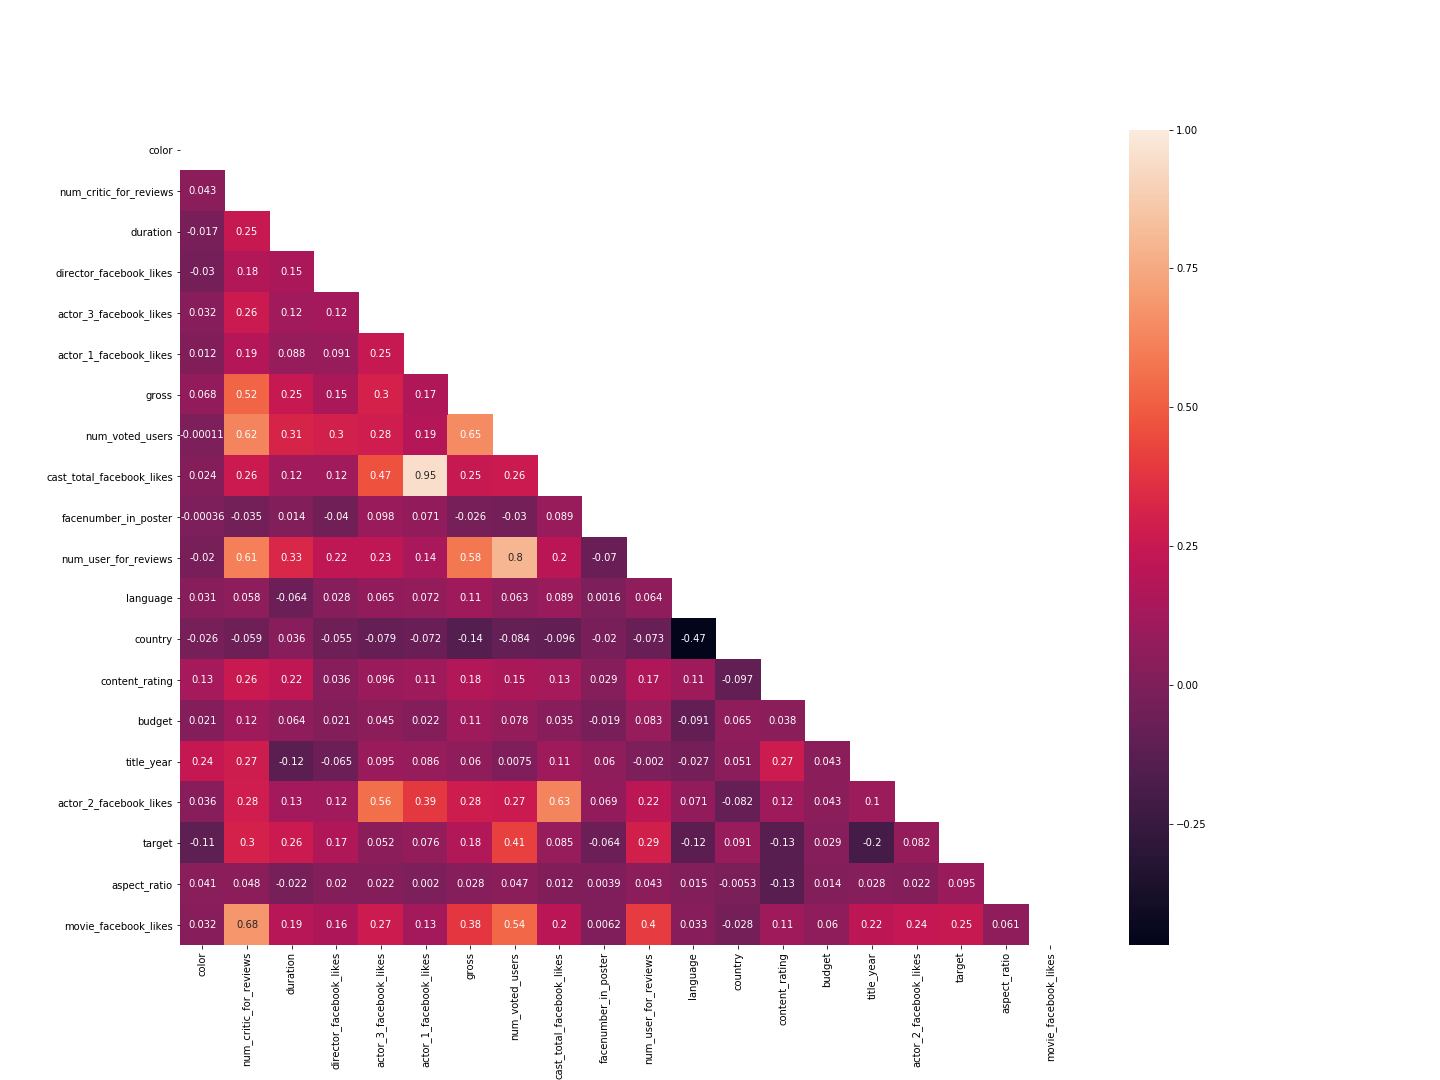
\includegraphics[height=15cm]{imagens/heatmap.png}
\caption{Heatmap}
\label{heatmap}
\end{figure}

A figura \ref{heatmap} representa um \textit{heatmap} (mapa de calor) que mostra o quanto os campos estão correlacionados. Por exemplo, se um campo \textbf{x} tem uma correlação positiva muito alta com o campo \textbf{y}, isso significa que quando o valor de um aumentar, o valor do segundo campo provavelmente também irá aumentar. Na figura acima, é possível notar que quanto maior a relação entre dois campos, mais claro o quadrado que exibe a relação fica no mapa. 
Na mesma figura é possível ver que existem campos com uma correlação maior com a nota (\textit{target}) como \textbf{num\_crit\_for\_reviews} e \textbf{num\_voted\_users}. 

É possível assumir que algumas colunas não são necessárias para a análise, como \textbf{imdb\_link}, que é apenas o \textit{link} do filme na página do IMDB e não tem relação nenhuma com a nota.

Alguns gráficos foram gerados para poder realizar uma análise mais profunda dos dados: 

\begin{figure}[H]
\centering
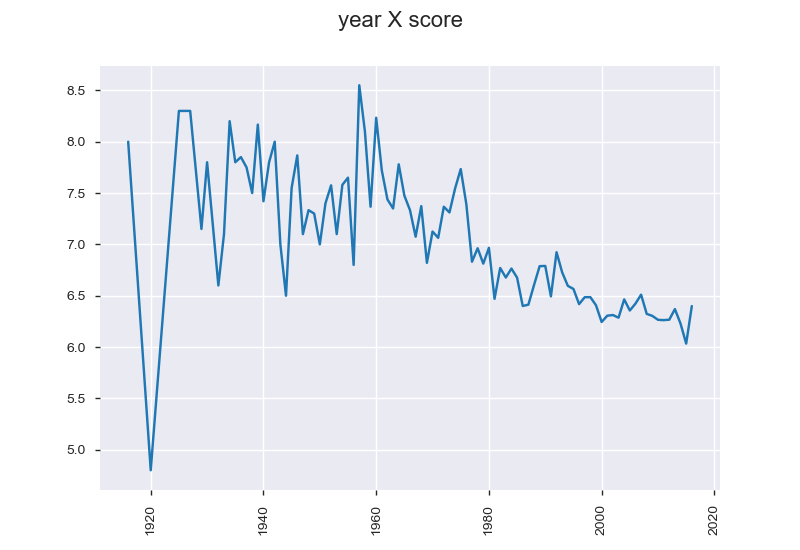
\includegraphics[height=10cm]{imagens/yearXscore.png}
\caption{Ano X Nota}
\label{yearXscore}
\end{figure}

Na figura \ref{yearXscore} é possível perceber que a média das notas veio caindo. Excetuando o ano de 1920, que teve uma média incrivelmente baixa, os anos seguintes se mantiveram entre 8.5 e 6.5. A partir da década de 80, o cenário começou a mudar e as médias começaram a baixar, chegando em 2016 (último ano que existe no \textit{dataset}) a aproximadamente 6.5.

\begin{figure}[H]
\centering
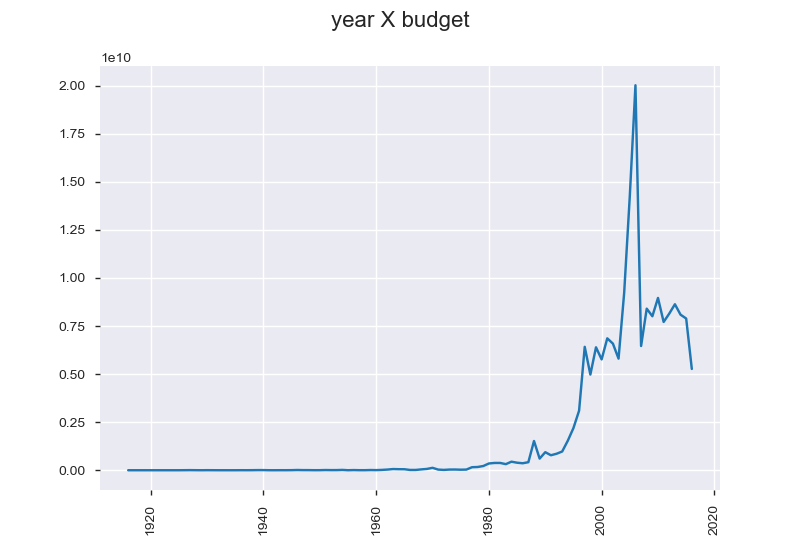
\includegraphics[height=10cm]{imagens/yearXbudget.png}
\caption{Investimento X Ano}
\label{budgetXyear}
\end{figure}
A figura \ref{budgetXyear} acima mostra que o investimento nos filmes aumentou consideravelmente. Entre a década de 90 e os anos 2000 teve um aumento quase exponencial.

\begin{figure}[H]
\centering
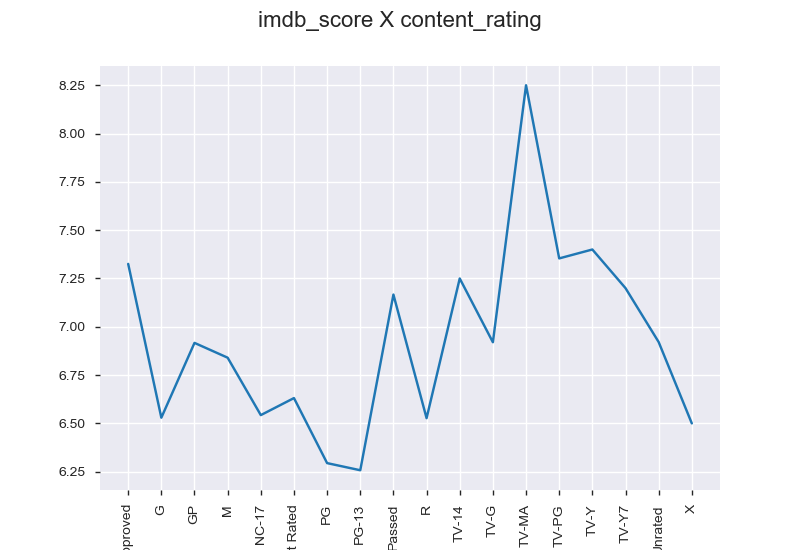
\includegraphics[height=10cm]{imagens/scoreXcontent.png}
\caption{Classificação indicativa X Nota}
\label{ratingXscore}
\end{figure}
Outra variável que pode influenciar a nota dos filmes é a classificação indicativa. A figura \ref{ratingXscore} mostra que filmes com a classificação \textbf{TV-MA} tendem a ter uma nota maior. Cerca de 2098 amostras encontradas nesses dados contêm a classificação \textbf{R}, porém a média das notas para esses filmes é de pouco mais de 6.5.

\subsection{Preparação dos dados}
Aqui os dados serão limpos, elevando a qualidade para realizar a análise.

\subsubsection{extract}
No primeiro passo do ETL, que é o de extração, \textit{extract}, os dados foram extraídos com auxilio do \pdi com um \textit{step} de \textit{read csv}, já que o arquivo é um csv. Existiu a necessidade de formatar corretamente os campos de números, e nos de texto foi necessário realizar uma operação \textit{trim} para remover espaços em brancos desnecessários, como mostra a figura \ref{extractProcess}. 

\begin{figure}[H]
\centering
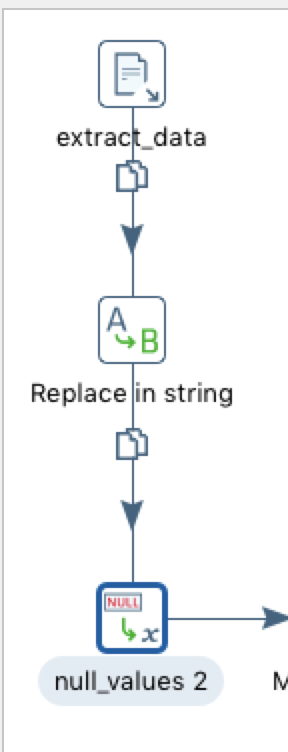
\includegraphics[height=3cm]{imagens/primeiro_tratamento.png}
\caption{Processo de \textit{extract}}
\label{extractProcess}
\end{figure}

\subsubsection{Transform}
O passo de \textit{transform} foi realizado com o auxílio da linguagem \textbf{Python} com as bibliotecas \textbf{pandas}, \textbf{sklearn}\footnote{https://scikit-learn.org/stable/} e \textbf{numpy}\footnote{http://www.numpy.org/} através do \textbf{Jupyter Notebook}\footnote{http://jupyter.org/}.

Os campos \textit{budget}, \textit{title\_year}, \textit{num\_critc\_for\_reviews}, \textit{duration}, \textit{actor\_1\_facebook\_likes}, \textit{actor\_2\_facebook\_likes},\textit{actor\_3\_facebook\_likes}, \textit{facenumber\_in\_poster}, \textit{num\_user\_for\_reviews}, que são campos de valores contínuos, tiveram seus valores vazios substituídos pela média. Esse tipo de substituição foi o suficiente por que a porcentagem de valores faltantes é muito baixa.

Em seguida, os valores nulos de campos textuais foram substituídos por n/a. Após esse passo, os campos \textit{actor\_1\_name}, \textit{actor\_2\_name},\textit{actor\_3\_name} e \textit{director\_name} foram substituídos por identificadores, tendo assim um range de valores discretos para ajudar no processo, como mostra a figura \ref{nullAndNames} abaixo.

\begin{figure}[H]
\centering
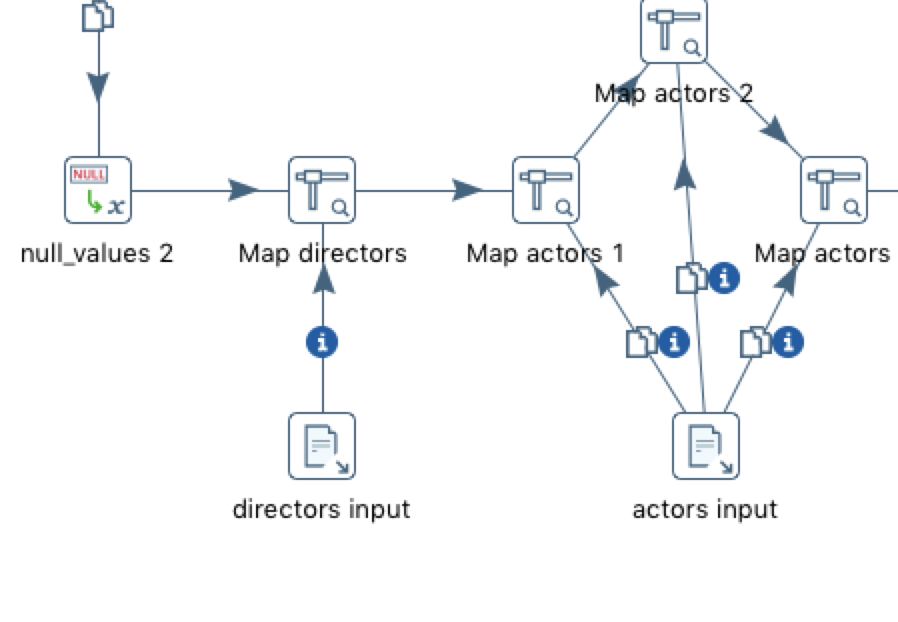
\includegraphics[height=7cm]{imagens/null_and_names.png}
\caption{Processo de \textit{transform} de campos}
\label{nullAndNames}
\end{figure}

A figura \ref{mappers} abaixo, mostra que os campos \textit{color, language, country, content\_rating} também foram substituídos para uma extensão de valores discretos.

\begin{figure}[H]
\centering
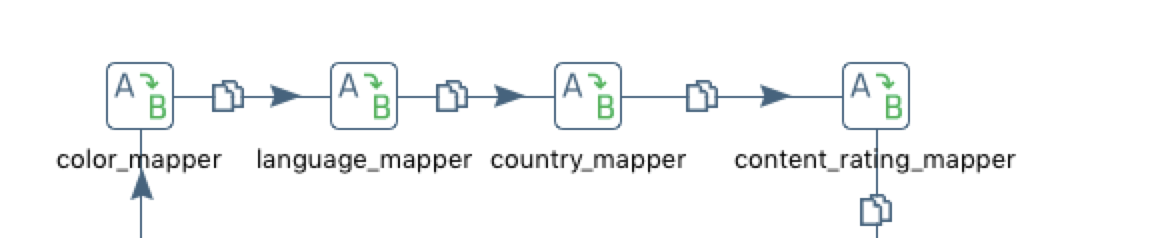
\includegraphics[height=3cm]{imagens/mappers.png}
\caption{Processo de \textit{transform} de campos}
\label{mappers}
\end{figure}

A coluna \textit{genres} no \textit{dataset} obtido inicialmente, está de uma forma que fica difícil de trabalhar. São apenas valores textuais exibidos da seguinte forma: "genero1|genero2|genero3". Isso pode dificultar o processo de aprendizado de máquina.

A figura \ref{genresDenormaliser} mostra os passos usados para tratar esse campo. A coluna foi removida e várias colunas com todos os gêneros encontrados foram criados. Caso o filme tenha o gênero, o campo correspondente fica com o valor 1, do contrario, valor 0.

\begin{figure}[H]
\centering
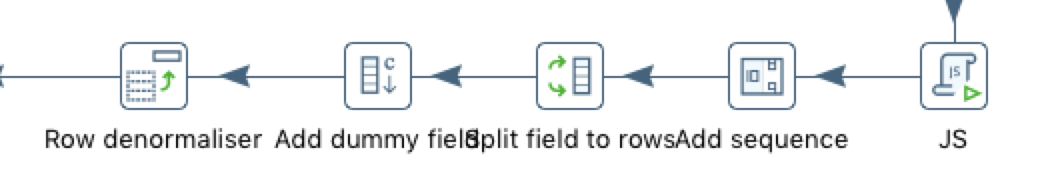
\includegraphics[height=3cm]{imagens/genres_step.png}
\caption{Processo de \textit{transform} de campos}
\label{genresDenormaliser}
\end{figure}

\subsubsection{Load}
O último passo, que é o carregar, \textit{load}, apenas carregou os dados em um outro arquivo csv, com o \textit{step text file output}, como mostra a figura \ref{lastStep}. Esse arquivo é usado mais tarde no WEKA.

\begin{figure}[H]
\centering
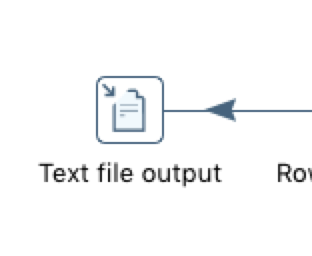
\includegraphics[height=2cm]{imagens/last_step.png}
\caption{Processo de \textit{load}}
\label{lastStep}
\end{figure}

\subsection{Objetivos}
O objetivo principal é prever a nota de um filme com base nos dados disponíveis e qual o nível de precisão.

Além disso, como dito anteriormente, outro objetivo que é determinar se os dados estão enviesados, já que contêm muitos filmes feitos nos Estados Unidos. Um outro é determinar se o diretor do filme tem grande influência sobre a nota dele. Também é possível verificar o quanto a nota do filme vai influenciar no lucro dele e o quanto o investimento feito pode influenciar a nota.

Após todos os passos acima, o próximo é realizar o processo de modelagem, levando em consideração todos os objetivos. Os dados foram carregados no WEKA e algoritmos de aprendizado de máquina foram usados. Um segundo \textit{dataset}, sem os filmes norte-americanos, foi criado e também carregado no WEKA, para validar ou não a afirmação feita de que os dados estão enviesados. 

Em resumo:

\begin{itemize}
    \item Prever nota de um filme com base nos dados disponíveis;
    \item A grande quantidade de filmes dos EUA adiciona um viés nos dados;
    \item Influência do investimento na nota;
    \item Influência do país na nota;
    \item Influência do diretor na nota;
\end{itemize}

\subsubsection{Modelagem}
As análises realizadas levaram em conta o RMSE, \textit{root mean squared error}, que calcula a raiz da diferença entre valor previsto e o valor real, como mostra a formula abaixo:

$RMSE = \sqrt{\frac{1}{n}\Sigma_{i=1}^{n}{\Big({predicted-actual}\Big)^2}}$
 
O MSE é muito usado em vários algoritmos porque ele tende a ser a medida mais fácil de ser manipulada matematicamente.

Em um primeiro momento, os dados gerados a partir do \pdi e as bibliotecas do \textit{Python} foram usados para selecionar o algoritmo de predição com os melhores resultados. Para isso, foram realizadas diversas análises com esses algoritmos no WEKA: os que tiveram o menor RMSE, tanto método de \textit{cross-validation} e o de 70\% split, foram \textit{linear regression}, \textit{bagging}, \textit{random committee} e \textit{random forest}, como mostra as tabelas abaixo:

\begin{longtable}{|l|l|l|}
\caption{Resultados da previsão usando \textit{cross-validation}}
\label{cvfull}
\\ \hline
\textbf{Algoritmo} & \textbf{RMSE}  \\ \hline
Linear Regression      & 0.827                    \\ \hline
Bagging                & 0.7685                   \\ \hline
Random Committee       & 0.7754                   \\ \hline
Random Forest          & 0.774                    \\ \hline
\end{longtable}


\begin{longtable}{|l|l|l|}
\caption{Resultados da previsão usando 70\% para treinamento e 30\% para teste}
\label{splitfull}
\\\hline
\textbf{Algoritmo} & \textbf{RMSE} \\ \hline
Linear Regression      & 0.8122                   \\ \hline
Bagging                & 0.7529                   \\ \hline
Random Committee       & 0.7468                   \\ \hline
Random Forest          & 0.7245                   \\ \hline
\end{longtable}


\subsubsection{Avaliação}
Para testar a hipótese de que a grande quantidade de filmes dos EUA adiciona um viés nos dados, os filmes feitos nos Estados Unidos foram removidos do \textit{dataset}. Ao remover esses filmes e também aplicar o algoritmo que teve os melhores resultados, o \textit{random forest}, ele retornou um RMSE de 0.7674 (figura \ref{nousacv}) com o método \textit{cross-fold validation} e 0.7341 (figura \ref{nousasplit}) usando o \textit{percentage split}. Os resultados não mudaram tanto, porém a quantidade de amostras sim, foram de 4998 para 1224. Talvez o filme ser do EUA tenha de fato influência sobre a nota final, porém não é possível definir com clareza somente com essa quantidade de dados, já que muita informação se perde.

\begin{figure}[H]
\centering
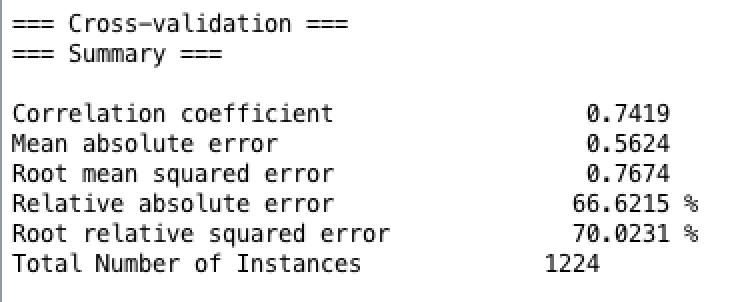
\includegraphics[height=5cm]{imagens/sem_usa_cv.png}
\caption{Sem filmes dos EUA e usando \textit{cross-validation}}
\label{nousacv}
\end{figure}

\begin{figure}[H]
\centering
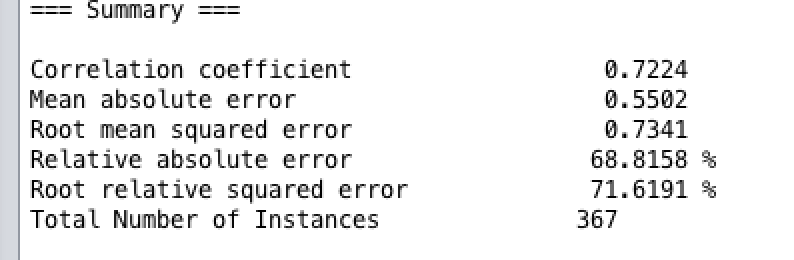
\includegraphics[height=5cm]{imagens/sem_usa_split.png}
\caption{Sem filmes dos EUA e usando \textit{percentage split}}
\label{nousasplit}
\end{figure}


Em seguida, a outra hipótese levantada é de que o investimento feito no filme tem influência na nota final. A figura \ref{nobudgetcv} mostra um RMSE de 0.7496, utilizando \textit{cross-validation} e a figura \ref{nobudgetsplit} mostra um erro de 0.7235. Mesmo o RMSE sendo um pouco menor, a diferença no erro entre os resultados obtidos nessa avaliação e com todos os dados, também é pequena demais para poder ser de alguma significância.

\begin{figure}[H]
\centering
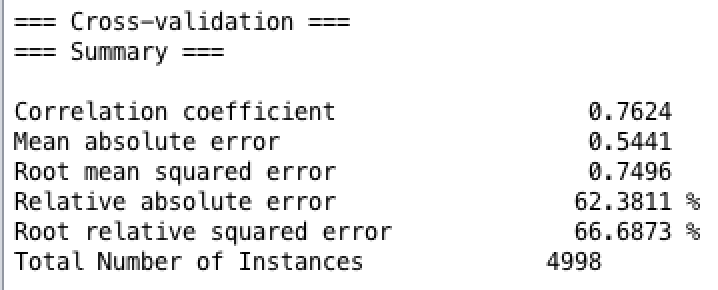
\includegraphics[height=5cm]{imagens/no_budget_cv.png}
\caption{Sem a coluna de orçamento e usando \textit{cross-validation}}
\label{nobudgetcv}
\end{figure}

\begin{figure}[H]
\centering
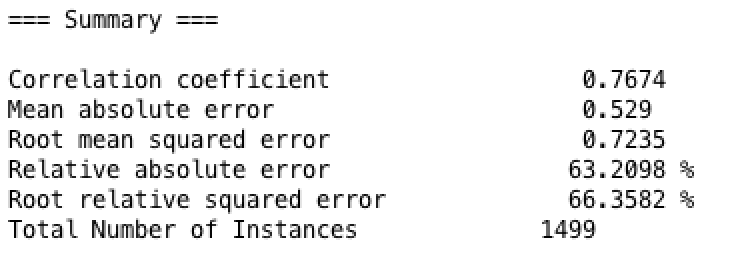
\includegraphics[height=5cm]{imagens/no_budget_split.png}
\caption{Sem a coluna de orçamento e usando \textit{percentage split}}
\label{nobudgetsplit}
\end{figure}


Uma outra hipótese é que o país vai ter influência nos resultados das notas dos filmes. Para testar essa afirmação, a coluna de países foi removida e o mesmo algoritmo citado anteriormente foi usado. A figura \ref{nocountrycv} mostra um RMSE de 0.7462, com \textit{cross validation}. Já a figura \ref{nocountrysplit}, que é com o método \textit{percentage split}, mostra um RMSE de 0.7313. Ao comparar os resultados do \textit{dataset} inteiro, é possível concluir que o país tem sim certa influência na nota, mas é muito pouca para ser significativa. 

\begin{figure}[H]
\centering
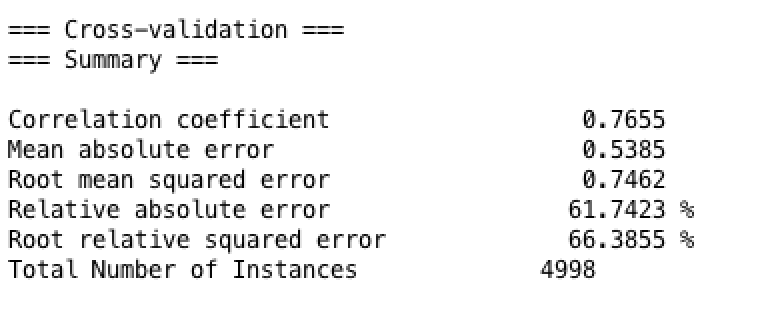
\includegraphics[height=5cm]{imagens/no_country_cv.png}
\caption{Sem a coluna de país e usando \textit{cross-validation}}
\label{nocountrycv}
\end{figure}

\begin{figure}[H]
\centering
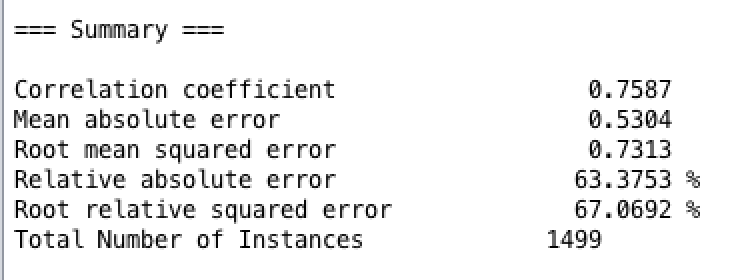
\includegraphics[height=5cm]{imagens/no_country_split.png}
\caption{Sem a coluna de país e usando \textit{percentage split}}
\label{nocountrysplit}
\end{figure}


Por último, a hipótese de que o diretor pode influenciar foi testada. Primeiro, com \textit{cross-validation} como mostra a figura \ref{nodirectorcv} tem um RMSE de 0.7451, já com \textit{percentage split}, tem um erro de 0.7264, como mostra a figura \ref{nodirectorsplit}. Com o método \textit{cross-validation} o erro foi menor, já com a técnica de \textit{percentage split} o RMSE foi um pouco maior, 0.0019. Isso mostra que o diretor escolhido para dirigir o filme não tem tanta influência na nota do filme. 

\begin{figure}[H]
\centering
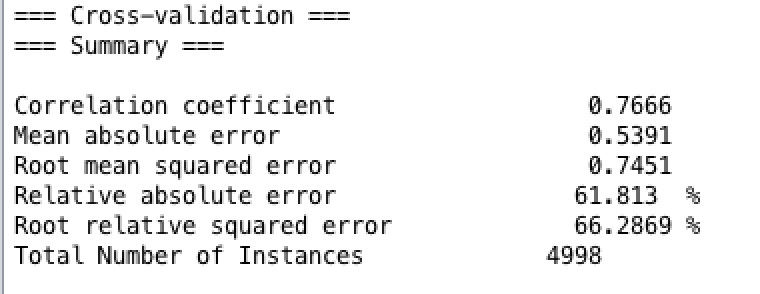
\includegraphics[height=5cm]{imagens/no_director_cv.png}
\caption{Sem a coluna de diretor e usando \textit{cross-validation}}
\label{nodirectorcv}
\end{figure}

\begin{figure}[H]
\centering
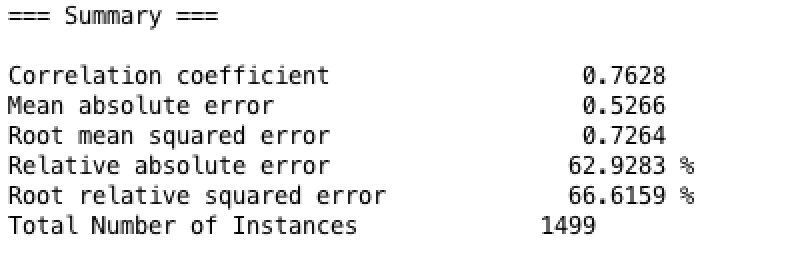
\includegraphics[height=5cm]{imagens/no_director_split.png}
\caption{Sem a coluna de diretor e usando \textit{percentage split}}
\label{nodirectorsplit}
\end{figure}

Dentre todas as hipóteses levantadas, apenas a primeira pôde ser testada com maior precisão, a de prever a nota dos filmes. Utilizando \textit{random forest} e realizando o tratamento dos dados descritos nessa seção, foi possível chegar a um RMSE de 0.7748, com \textit{cross-validation} (tabela \ref{cvfull}) e 0.7245 usando \textit{percentage split} (tabela \ref{splitfull}). 

Diante disso, o trabalho aqui realizado foi capaz de prever as notas com um erro relativamente baixo, de aproximadamente 0.7245, usando \textit{percentage split}. Foi difícil saber com certeza se outros atributos tinham uma influência direta no resultado final, visto que a variação no resultado era muito pouca. Removendo individualmente os atributos de país, diretor e orçamento, o RMSE final variou muito pouco, fazendo com que qualquer conclusão seja imprecisa.

Não foi possível definir se os dados estavam ou não enviesados sem uma observação maior deles, já que o erro, no caso da análise sem os filmes feitos nos Estados Unidos, foi menor. Além de que, sem as produções feitas nos EUA, a quantidade de registros cai de 4998 para 1224, perdendo muitos dados que são de grande importância para a análise de regressão.

A tabela \ref{results} mostra os resultados obtidos:

\begin{longtable}{|l|l|l|}
\caption{Resultados Obtidos}
\label{results}
\\\hline
\textbf{Análise} & \textbf{\% split} & \textbf{Cross Validation} \\ \hline
Todos os dados      & 0.7245    & 0.774               \\ \hline
Sem filmes dos EUA      & 0.7341    & 0.7674               \\ \hline
Sem Orçamento         & 0.7235     & 0.7496              \\ \hline
Sem País         & 0.7313     & 0.7462              \\ \hline
Sem Diretor         & 0.7264     & 0.7451              \\ \hline
\end{longtable}

\section{Conclusões}
Neste trabalho, foi explicado o que é um \textit{Data Warehouse}, os tipos, tipos de operação. Também foi explicado o que é o processo de ETL. Uma das ferramentas que auxiliou no processo de ETL \pdi foi apresentada. Outra ferramenta apresentada foi o WEKA, que auxilio no processo de aprendizado de máquina. Foram também apresentados conceitos de CRISP-DM e \textit{Data Mining}.

Em seguida foi apresentado o estudo de caso, onde foi feita uma análise exploratória dos dados, foi mostrado como o processo de ETL foi aplicado, quais hipóteses foram levantadas e os resultados dessas hipóteses. 

A partir delas, foi possível prever a nota de filmes com um RMSE relativamente pequeno, porém que pode ainda ser melhorado. Uma das formas de reduzir ainda mais, é gerando mais atributos derivados. Também não foi possível afirmar que os dados estavam enviesados.

Um sistema de recomendações utilizando os resultados desse trabalho é uma possível extensão desse projeto. O sistema poderia levar em consideração a nota que o usuário deu para certos filmes e os gêneros deles, podendo indicar um com uma chance maior de acerto, ou seja, de agradar o usuário. Além disso, o sistema poderia ajudar a escolher pessoas atrizes que têm uma maior influência nas notas, evitando fazer uma escolha possivelmente ruim.
%%%%%%%%%%%%%%%%%%%%%%%%%%%%% Referências 

\nocite{*}
\bibliography{references} 
\bibliographystyle{plain}
%%%%%%%%%%%%%%%%%%%%%%%%%%%%%%%%%%%%%%%%%%%%%%%%%%%%%%%%%%%%%%%%%%%%%%%


\end{document}